\section{Teil}
beinhaltet folgende Foliensätze:

\begin{itemize}
    \item Teil 4:  Systemverhalten (Grundlagen der Modellplanung und –Bildung und Simulation)

\end{itemize}

% subsection
%-------------------------------------------------------------------------------------------
\subsection{Was ist ein Modell?}
Modelle sind Abstraktionen und Vereinfachung der Realität und zeigen deshalb nur Teilaspekte auf.
Es ist daher wichtig, dass die Modelle im Hinblick auf die Situation und die Problemstellung aussagekräftig sind.
Dies bedeutet, dass bei allen Überlegungen die Frage nach der Zweckmäßigkeit und der Problemrelevanz zu stellen ist.
\begin{figure}[H]
    \centering
    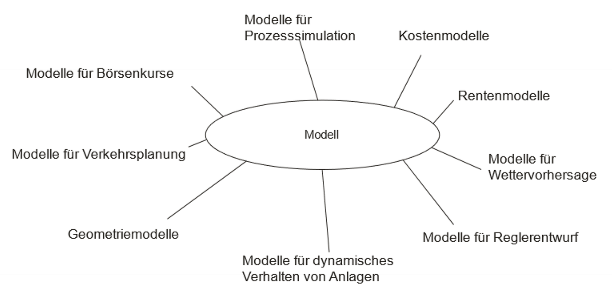
\includegraphics[width=0.6\linewidth]{Bilder/Teil4_ModelleBeispiel1.png}
    \caption{Beispiel Modelle verschiedener Lebensbereiche}
\end{figure}
% subsection
%-------------------------------------------------------------------------------------------
\subsection{Was bedeutet Problemlösung durch Abstraktion (Modellbildung) und Interpretation?}
\begin{figure}[H]
    \centering
    \includegraphics[width=0.6\linewidth]{Bilder/Teil4_ProblemlösungdurchAbstraktionundInerpretation.png}
    \caption{Problemlösung durch Abstraktion und Interpretation}
\end{figure}

% subsection
%-------------------------------------------------------------------------------------------
\newpage
\subsection{Welche Verfahren der Modellbildung gibt es?}
\begin{itemize}
    \item \textbf{Rechnerische Verfahren:}\\
    Dazu werden \textbf{mathematische Modelle} benötigt, die formal durch \textbf{Gleichungen} (algebraisch oder differenzial)
    beschrieben werden, zu deren Lösung heute neben den traditionellen analytischen Verfahren leistungsfähige numerische und 
    symbolische Softwareprogramme zur Verfügung stehen.
    \item \textbf{Experimentelle bzw. messtechnische Verfahren:}\\
    Zu ihrer ANwendung werden \textbf{physikalische (experimentelle) Modelle} benötigt, an denen Versuche, Messungen und Auswertungen
    durchgeführt werden können. Im Maschinenbau etwa sind dies typischerweise Prototypen, Testobjekte, VErsuchsanordnungen oder
    maßstäbliche Modelle. Mit Hilfe der physikalischen Modelle sollen alle wesentlichen Einflüsse "messtechnisch" erfasst werden.
    \item \textbf{Hybride Verfahren} (Kombination von Berechnung und Experiment bzw. Messung):\\
    Diese Verfahren \textbf{nutzen sowohl Messgrößen as auch mathematische Modelle.} Während bei rechnerischen Verfahren Fehler aufgrund
    von Modellierungsungenauigkeiten auftreten, sind bei experimentellen Verfahren mehr oder weniger große Messfehler unvermeidbar.
    Liegen sowohl mathematische Modelle als auch Messergebnisse vor, so kann man versuchen, Hypothesen über die Art der Fehler 
    zu bilden und das Modell anhand der Messergebnisse zu verbessern, dass sich eine bessere Übereinstimmung von Rechnung und 
    Experiment ergibt.
\end{itemize}

% subsection
%-------------------------------------------------------------------------------------------
\subsection{Wie ist der Ablauf zur Entstehung eines rechnerinternen Modells?}
\begin{itemize}
    \item Der Modellbildner entwickelt eine gedankliche Vorstellung des zu untersuchenden Originals (z.B. eines realen 
    technischen objekts oder eines neuen Produkts) in Form eines mentalen Modells (Gedankenmodells), das anschließend 
    zu einer Erfassung in eine formalisierte Informationsform mit Hilfe von Informationselementen und -strukturen gebracht wird.
    \item Dieses \glqq Informationsmodell\grqq wird am Rechner implementiert (rechnerinternes Modell).
\end{itemize}
\begin{figure}[H]
    \centering
    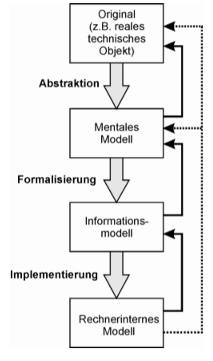
\includegraphics[width=0.3\linewidth]{Bilder/Teil4_RechnerinternesModell.png}
    \caption{Ablauf zur Entstehung eines rechnerinternen Modells}
\end{figure}

% subsection
%-------------------------------------------------------------------------------------------
\subsection{Was ist bei der Interpretation von Ergebnissen wichtig?}
Eine wichtige Aufgabe des Produktentwicklers (Versuchstechnikers, Berechnungsingenieurs) ist die 
Interpretation der Ergebnisse. Dazu muss er zwischen physikalischen Phänomenen und künstlichen Effekten 
(Artefakten), die z.B. von Messfehlern bzw. numerischen Lösungsverfahren herrühren, unterscheiden können. Dies 
erfordert Kenntnisse und Erfahrung sowohl über die untersuchten Fragestellungen als auch über die (z.B. 
versuchstechnischen bzw. numerischen) Verfahren, die zur Lösung des Modellproblems verwendet werden. Einfache, 
überschlägige Abschätzungen und Erfahrung sind unerlässlich, um die Ergebnisse (Messergebnisse bzw. Rechenergebnisse) 
zu überprüfen sowie zu bewerten und damit hohe Qualität der Simulation sicherzustellen.

% subsection
%-------------------------------------------------------------------------------------------
\subsection{Was bedeutet Simulation und wofür ist dies relevant?}
In der VDI-Richtlinie 3633 mit dem Titel „Simulation von Logistik-, Materialfluss- 
und Produktionssystemen – Begriffsdefinitionen“ [VDI-3633] ist Simulation wie folgt definiert:
\begin{itemize}
    \item  Simulation ist ein Verfahren zur Nachbildung eines Systems mit seinen 
    dynamischen Prozessen in einem experimentierbaren Modell, um zu 
    Erkenntnissen zu gelangen, die auf die Wirklichkeit übertragbar sind. Im 
    weiteren Sinne wird unter Simulation das Vorbereiten, Durchführen und 
    Auswerten gezielter Experimente mit einem Simulationsmodell verstanden. Mit 
    Hilfe der Simulation kann das zeitliche Ablaufverhalten komplexer Systeme 
    untersucht werden (Simulationsmethode).    
\end{itemize}
Simulationen werden dann durchgeführt wenn:
\begin{itemize}
    \item kein reales System verfügbar ist (Entwurfsphase)
    \item das Experiment am realen System zu lange dauert
    \item das Experiment am realen System zu teuer ist
    \item das Experiment am realen System zu gefährlich ist (Flugzeug, Kraftwerk)
    \item die Zeitkonstanten des realen Systems zu groß sind (Klimamodelle)
\end{itemize}